\documentclass[12pt,a4paper]{article}
\usepackage{times}
\usepackage{durhampaper}
%\usepackage{harvard}
\usepackage{tikz}
\usepackage{tabularx}
\usepackage{placeins}

%\citationmode{abbr}
%\bibliographystyle{agsm}
\bibliographystyle{apalike}

\title{Tailoring Horror Games with Biometrics}
\author{David Budgen}
\student{Steven Lowes}
\supervisor{Magnus Bordewich}
\degree{BSc Computer Science}

\date{2019-01-25}

\begin{document}

\maketitle

\begin{abstract}
%These instructions give you guidelines for preparing the design paper.  DO NOT change any settings, such as margins and font sizes.  Just use this as a template and modify the contents into your design paper.  Do not cite references in the abstract.

%The abstract must be a Structured Abstract with the headings {\bf Context/Background}, {\bf Aims}, {\bf Method}, and {\bf Proposed Solution}.  This section should not be no longer than a page, and having no more than two or three sentences under each heading is advised.

\textbf{Context/Background}
Horror games are a large industry, with thousands of games and hundreds of millions of copies owned. Players are thrilled by experiencing fear in a safe and secure environment. However, each player reacts differently and the one-size-fits-all approach can prove constricting for players.

\textbf{Aims}
The project aims to explore how biometrics can be integrated into horror games to improve the user's experience by adjusting gameplay based on data readings. A secondary aim of the project is to make developing a horror game easier by removing the need to pre-program scare locations in an environment.

\textbf{Method}
A simple horror game with the ability to read data from sensors will be created. The rate and timing of scares will be adjusted based on the sensor data, and a user study will be conducted to explore whether the biometrics improve the gameplay experience. The `Biometric' method will be compared to a `Random' method which is not based on the sensor readings.

\textbf{Proposed Solution}
The game Minecraft will be modified to add a jump-scare which can be triggered programmatically. After a jump-scare is activated, the system will read data from an EDA sensor and allow more time between scares if it believes that the user is becoming desensitized. This Biometric algorithm will be compared to a Random algorithm which scares at random intervals.
\end{abstract}

\begin{keywords}
Biometrics, Biosensors, Electrodermal Activity, Human-Computer Interaction, Video Games, Horror
\end{keywords}

\section{Introduction}
%This section briefly introduces the project, the research question you are addressing.  Do not change the font sizes or line spacing in order to put in more text.

%Note that the whole report, including the references, should not be longer than 12 pages in length (there is no penalty for short papers if the required content is included). There should be at least 5 referenced papers.

\subsection{Horror Games}
The horror games industry is huge, with over 2000 unique titles on steam and almost 500 million copies owned \cite{horrorSteamSpy}. The vast majority of these games present the same experience to all players, though there have been experiments in tailoring the games to the individual. Games such as  \emph{Nevermind} \cite{nevermind}, and \emph{Bring to Light} \cite{bringtolight} both allow the use of heart-rate monitors to adjust gameplay.

The use of heart rate monitors in these games is not ideal, but makes sense for a mass-market game as heart rate sensors are some of the most widely available biometric sensors. Heart rate sensors are limited as they struggle to show the immediate response to a scare. They can tell how scared a person is, but not how scared an individual event made them. In contrast, this project will use EDA sensors which can detect changes on the order of milliseconds, making them an ideal feedback mechanism in a horror game \cite{edaAnalysis}.

Horror games are perfect for measuring with biometrics, as we have a defined event which we know will cause a large reaction, and we can use the sensors to measure the response to that known event. This is similar to with a lie detector - we have an event (a person answering a question) and we want to see whether it caused a response. This is much simpler than trying to detect stress over a long period as the timing of the known stimulus can be used to predict a change in biometrics.

\subsection{Biometrics}
Biometrics are becoming increasingly ubiquitous. 67\% of smartphones include a fingerprint scanner \cite{fingerprint}, and 141 million smartwatches were sold in 2018 \cite{smartwatches}, nearly all of which are constantly taking heart-rate measurements.

Consumers are increasingly becoming accustomed to the fact that wearable tech and biometrics can be used to improve their user experience. Despite this, biometrics have seen little use in the entertainment industry.

As biometrics become more accepted and more integrated, they will allow for a new step in human-computer interfacing. Just as the inclusion of a fingerprint sensor allowed smartphones to identify their user autonomously, integrated sensors will allow applications to get immediate feedback without the user having to switch contexts and give a rating. This means that they can iteratively improve without user or developer intervention. Eventually, these biometrics will extend to the point of brain-computer interfacing, where the program can adjust to the individual tastes and preferences of the user without having to test the available options individually.

\subsection{Physiological Arousal and EDA}
Physiological arousal is a measure of how alert the body is. It can be caused by intense emotion, shock, or surprise, and is strongly linked to the `fight or flight' reflex. When experiencing high arousal, the body's blood pressure and heart rate increases, readying the body to respond to a stimulus \cite[pp.162-167]{arousal}.

When the body is becoming more aroused, it leads to an increase in `Electrodermal Activity' (EDA). EDA is a measure of how much the body is sweating, and is measured by testing the resistance between two electrodes. When the participant experiences high EDA, the resistance between the electrodes decreases \cite[pp.2-3]{eda}. GSR is a synonymous (though outdated) term for EDA, which is notably used in the name of the EDA sensor that the system uses.

EDA is used in many applications, including as part of the polygraph (lie-detector) test, where it can detect the physiological arousal caused by lying and being afraid of the repercussions of doing so \cite{polygraph}. It is also used by the `Church of Scientology' to guide therapy in removing any negative associations from words and concepts, a controversial technique known as `auditing' \cite[p.32]{auditing}.

The EDA response consists of a sharp drop in resistance, over a period of {\raise.17ex\hbox{$\scriptstyle\sim$}}1s, when arousal passes a certain threshold (the size of the drop correlates with the extent of the arousal), followed by an asymptotic increase in resistance back to a high base value, with a half-life of {\raise.17ex\hbox{$\scriptstyle\sim$}}10s. The initial drop occurs 1-3 seconds after the stimulus. That high base value is rarely reached because arousal varies frequently even without any explicit stimulus, so the EDA response happens quite often \cite{edaAnalysis}.

\subsection{Project Purpose}
This study will explore whether users show any preference between a horror game where jump scares are randomly allocated and the same game where jump scares are tailored based on biometric feedback. An extensive user study will be conducted and the results analysed to explore the difference in self-reported user enjoyment and data gathered from biometrics measuring how scared the users were.

\subsection{Deliverables}
The following deliverables were decided upon to help achieve the project purpose:
\begin{enumerate}
	\item Minimum Deliverables
	\begin{itemize}
		\item Create an immersive game environment in which you can control events such as the arrival of new enemies and their location.
		\item Create a system for tracking the user EDA measurements and game events simultaneously.
		\item Create a standardised game setting for users to play through and record EDA measurements as they progress. Record some user experiences.
		\item Determine what game events trigger responses and select events to use in the next deliverables.
	\end{itemize}
	
	\item Intermediate Deliverables
	\begin{itemize}
		\item Analyse data from users and try to determine susceptibility to expected new shock events, e.g. underlying tension or delay since last event.
		\item Create one or more Biometric systems for triggering events at moments of maximum impact.
		\item Create a (null hypothesis) system for random generation of events.
	\end{itemize}
	
	\item Advanced Deliverables
	\begin{itemize}
		\item Conduct a user study to determine whether the Biometric algorithm gives a better user experience than the Random algorithm.
		\item Revise the Biometric algorithm based upon empirical evidence obtained.
	\end{itemize}
\end{enumerate}

\subsection{Prior Work}
The original plan for this project was to explore the use of EDA to find relaxing music. By representing songs as 14-dimensional vectors, where each component of the vector was a high-level quality of the song such as `acousticness' or `danceability', the problem could be treated as an AI search problem. Each song can be assigned a fitness based on how relaxing a user finds it when listening to it. The problem becomes to simply explore the 14-dimensional space of all songs and find the song with highest fitness.

However, there were two problems which meant that this project was entirely infeasible. Firstly, calculating the fitness of a song took the length of the song to do, since a human needed to listen to the song. To find a near-optimal solution in the dataset of 25 million songs that was used would take thousands of songs, which would mean weeks of music listening.

Secondly, it was discovered that the EDA sensor was a poor choice for the task of measuring how relaxing music was. For many of the reasons that EDA is a great choice for horror games, it is a terrible choice for music. There is no single stimulus that can be measured, meaning that it's impossible to decide whether a change in EDA was caused by the music or, for example, the user seeing a bird out of the window. In addition to this, EDA tends to drift over time, causing measurements to be thrown off by the temperature of the room and how hungry the user was. When working with a single stimulus, such as in horror games, the recording length is not long enough for this to cause an issue.

\subsection{Potential Impact}
This work could act as a launching point for other games integrating the use of sensors. With smartwatches becoming increasingly ubiquitous, in the future many games could access the sensors in those smartwatches to adjust gameplay. Sensor-enabled gameplay adjustment could be applied to other forms of entertainment. For example, action games could integrate biometrics by enabling slow-motion after detecting high-adrenaline moments. Games could further integrate biometrics as a central mechanic, i.e. in order to continue through the game you must learn to control your body's semi-autonomous responses. This tight integration of biometrics would allow for a new paradigm in computer entertainment.

Ultimately, this work aims to validate that the use of biometrics can lead to an improved gameplay experience, utilising horror games as the most ideal scenario during this exploratory phase.

\section{Design}
%This section presents the prohttps://steamspy.com/tag/horrorposed solutions of the problems in detail. The design details should all be placed in this section. You may create a number of subsections, each focusing on one issue.

%This section should be up to 8 pages in length.

%The rest of this section shows the formats of subsections as well as some general formatting information.  You should also consult the Word template.

%The font used for the main text should be Times New Roman (Times) and the font size should be 12.  The first line of all paragraphs should be indented by 0.25in, except for the first paragraph of each section, subsection, subsubsection etc. (the paragraph immediately after the header) where no indentation is needed.

%In general, figures and tables should not appear before they are cited.  Place figure captions below the figures; place table titles above the tables.  If your figure has two parts, for example, include the labels ``(a)'' and ``(b)'' as part of the artwork.  Please verify that figures and tables you mention in the text actually exist.  make sure that all tables and figures are numbered as shown in Table \ref{units} and Figure 1.

%sort out your own preferred means of inserting figures

The design of this project is split into four main categories which will be explored in order. Firstly, the requirements of the system will be defined and will proceed to guide every other aspect of the design. Then, the game environment and jump scares will be set out, defining the environment that players find themselves in. Following that, the behind-the-scenes design will be discussed, encompassing the software-engineering aspects of system design, and the actual algorithms that are being compared. Finally, the user study and experimental methodology, including ethical implications, will be explained.

\subsection{Requirements}
The requirements (on the following page) were decided upon to help guide the system through its design. They explain the fundamental aspects that need to be achieved by the design before we can begin a full user study.

\begin{figure}[!htbp]
	\begin{center}
		\begin{tabularx}{\linewidth}{c|Xc}
			\textbf{ID} & \textbf{Requirement} & \textbf{Priority}\\\hline
			FR1&Players can explore a spooky environment on their own&H\\
			FR2&Jump scares can be triggered at any time programatically&H\\
			FR3&The user's EDA can be measured over a period of time&H\\
			FR4&EDA data over a period can be reduced to a scalar value indicating how scared the user was&H\\
			FR5&The EDA measurements should be saved to a file&H\\
			FR6&Game environment can be reset with one command after each playtest&M\\
			FR7&Music should play during a playtest and should be configurable&M\\
		\end{tabularx}
		\caption{Functional Requirements}
	\end{center}
\end{figure}

\begin{figure}[!htbp]
	\begin{center}
		\begin{tabularx}{\linewidth}{c|Xc}
			\textbf{ID} & \textbf{Requirement} & \textbf{Priority}\\\hline
			NF1&The mod existing should not adversely affect gameplay (i.e. no increased lag)&H\\
			NF2&The sensor must not cause any harm to users. This is a concern due to the use of electrical currents, but the device is certified to be safe to use&H\\
			NF3&The user's aim during the playtest should be shown on the screen at the start and not be longer than 1 sentence&H\\
		\end{tabularx}
		\caption{Nonfunctional Requirements}
	\end{center}
\end{figure}

\FloatBarrier

\subsection{Choice of Game \& Environment}
The game Minecraft was chosen due to its comprehensive modding API, cross-platform compatibility, and ease of use when it comes to creating and exploring environments. It is simple for players and uses very standard controls, so most people will intuitively understand how to explore the environment. The modding API, named `Forge',  incredibly complete and mature despite being community-maintained and open-source. It has been in 
active development since 2011 \cite{ForgeGit}. 

Players will be placed in a purpose-built haunted house environment, chosen due to the typical horror game connotations. They will be given the goal of finding a number of items throughout the house, but will not be able to complete the task within the 10-minute time limit. This ensures that the users have a purpose and continue to explore the environment rather than staying in one location.

\subsection{Jump Scares}
On the following page is a screenshot of the jump-scare in action. A `creeper' face appears large on the screen, taking up most of the user's field of view. The creeper is a monster in Minecraft and has a reasonably scary appearance. At the same time, a loud noise plays. The noise consists of many in-game noises pitch-shifted and played at the same time. It is has many low frequencies and some high-pitched scream-like sounds. The waveform and spectogram of the noise follow as figures.

Even very non-scary jump scares cause a clear change in EDA. For example, on the following page is a graph of the EDA data while watching a screen that turns from black to white with the word `boo'. This very non-threatening scare caused a clear response, so I'm not concerned about there needing to be any actual risk of dying while playing the game. In fact, adding the ability to die from the jump scare could cause unnecessary random noise in the data. When the player has a higher risk of dying, they will show a more extreme response, regardless of the timing of the scare. Since the system has no idea of the player's environment when picking when to scare them, we want to remove that as a factor in how scared they are.

\begin{figure}[!htbp]
		\begin{center}

\includegraphics[width=0.8\linewidth]{scare.png}
\caption{The jump scare}
	\end{center}
\end{figure}

\begin{figure}[!htbp]
		\begin{center}
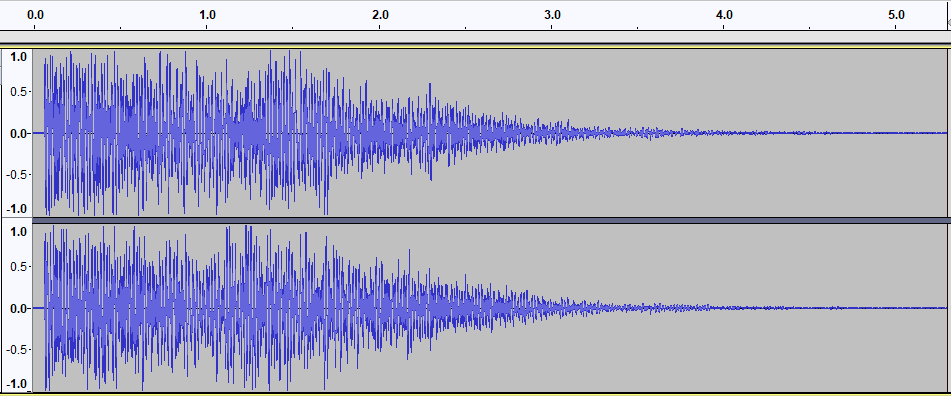
\includegraphics[width=0.8\linewidth]{waveform.png}
\caption{The waveform of the scary noise}
\end{center}
\end{figure}

\begin{figure}[!htbp]
		\begin{center}
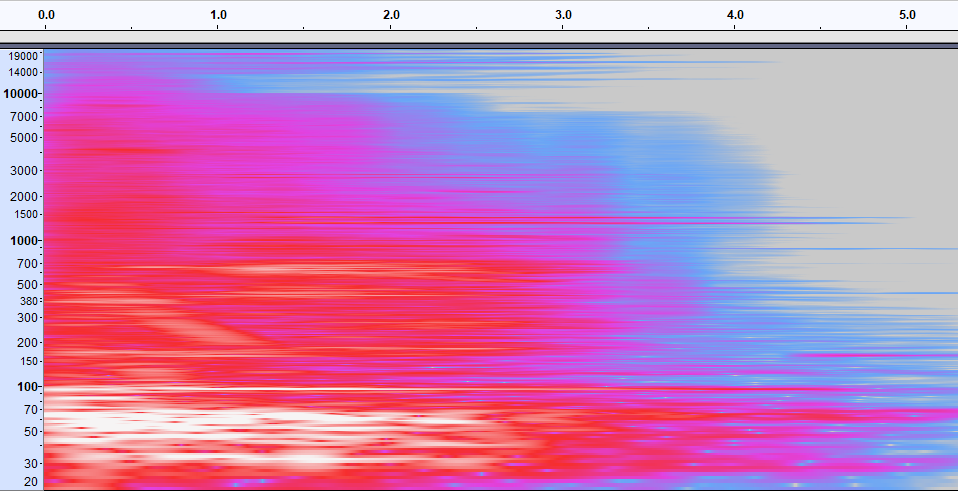
\includegraphics[width=0.8\linewidth]{spectogram.png}
\caption{The spectogram of the scary noise}
\end{center}
\end{figure}

\begin{figure}[!htbp]
	\begin{center}
	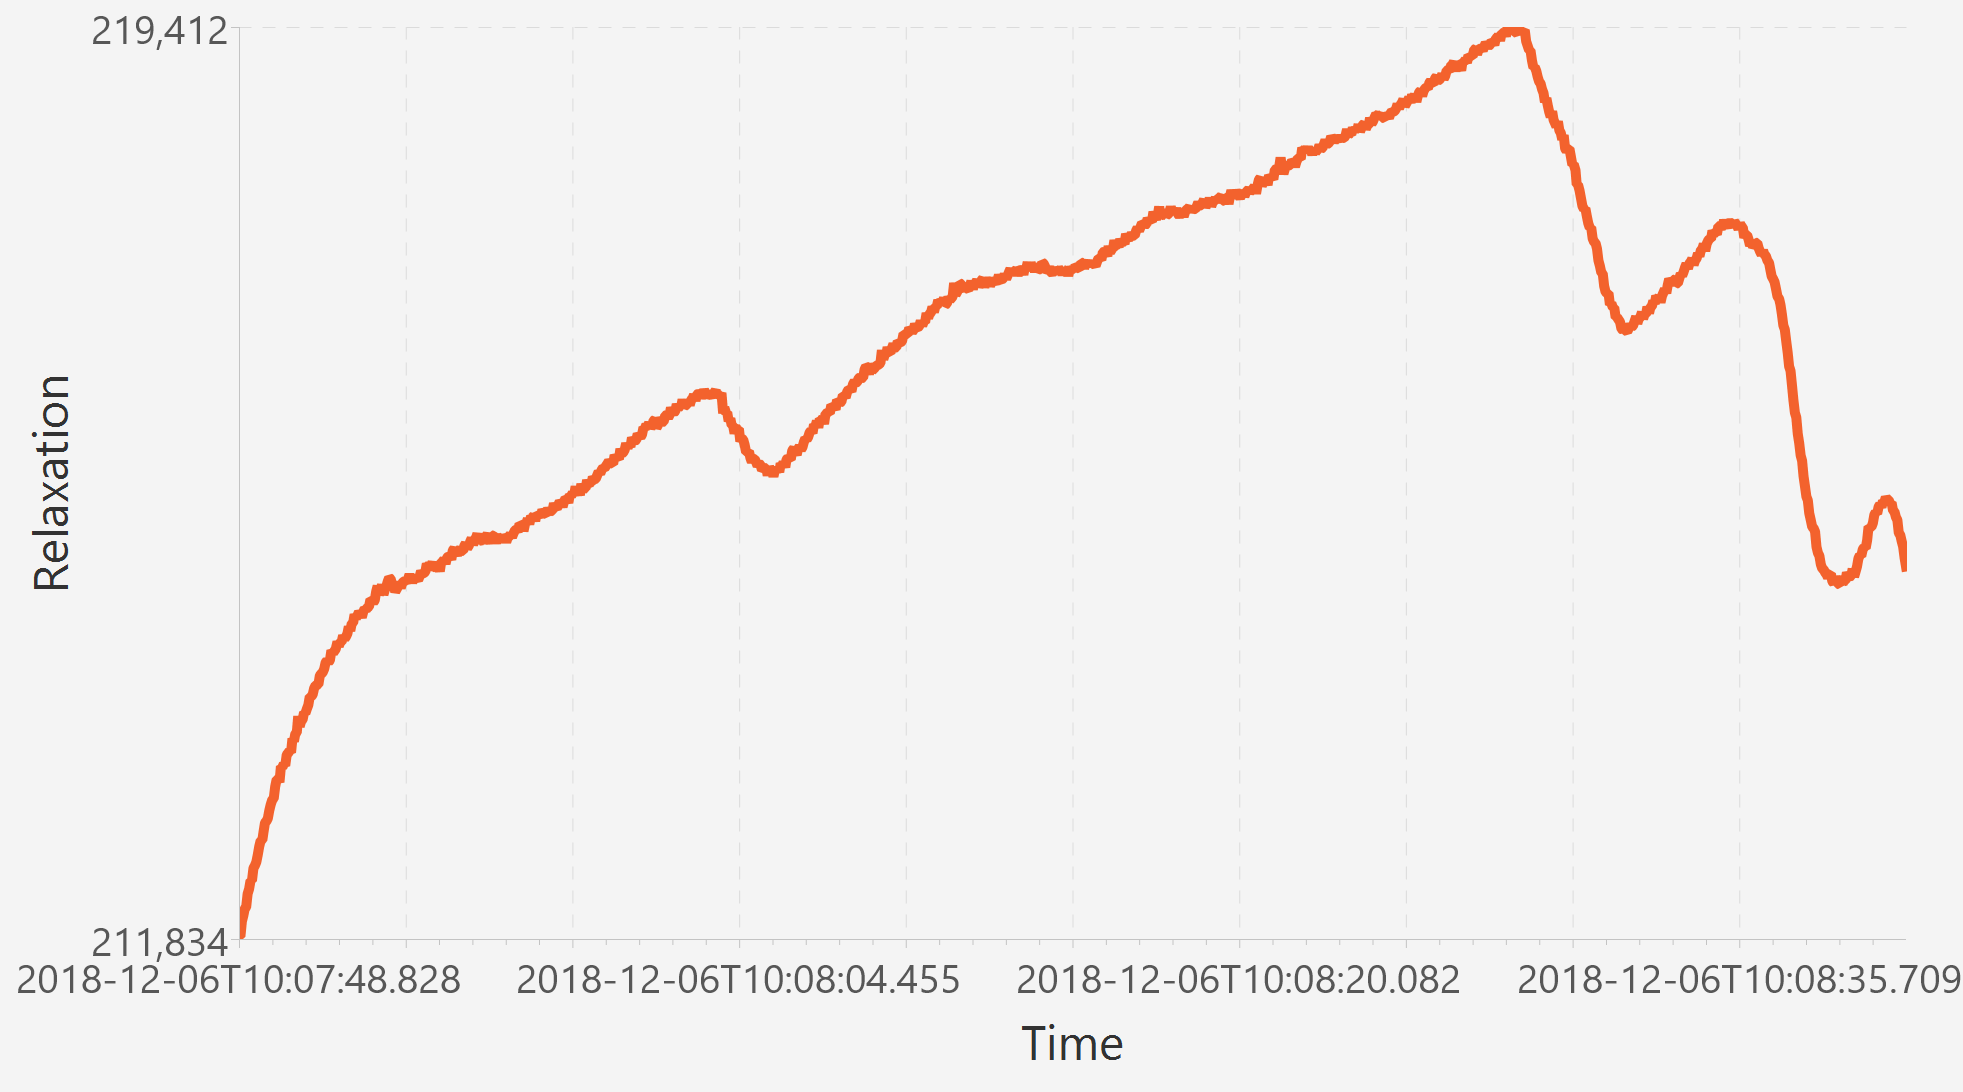
\includegraphics[width=0.8\linewidth]{boo.png}
	\caption{EDA data from a very non-scary jump scare}
\end{center}
\end{figure}
\FloatBarrier

\subsection{System Architecture}
\begin{figure}[!htbp]
	\begin{center}
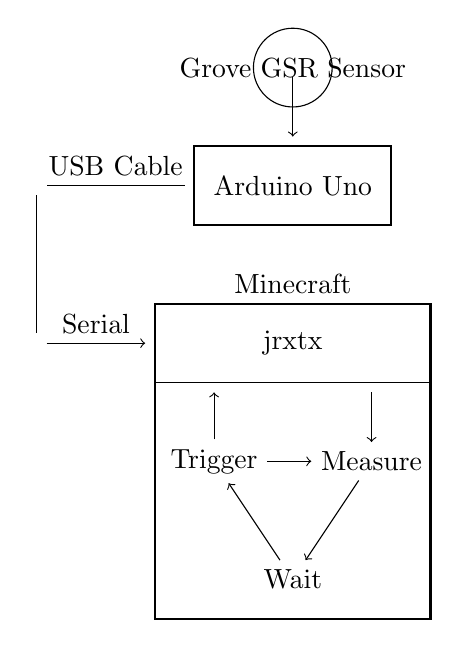
\begin{tikzpicture}
\draw  [thick](-0.5,0.5) rectangle (-3,-0.5);
\node at (-1.75,0) {Arduino Uno};
\node (v6) at (-1.75,0.5) {};
\node at (-1.75,1.5) {Grove GSR Sensor};
\draw  [thick](-3.5,-1.5) rectangle (0,-5.5);
\node (v8) at (-3,0) {};
\node (v7) at (-3.5,-2) {};
\node (v4) at (-5,0) {};
\node (v5) at (-5,-2) {};
\draw  (v4) edge (v5);
\draw  [->] (v5) edge (v7);
\draw  (v8) edge (v4);
\node at (-4,0.25) {USB Cable};
\draw  (-3.5,-1.5) rectangle (0,-2.5);
\node at (-1.75,-2) {jrxtx};
\node at (-1.75,-1.25) {Minecraft};
\node (v9) at (-1.75,-5) {Wait};
\node (v10) at (-2.75,-3.5) {Trigger};
\node (v11) at (-0.75,-3.5) {Measure};
\node (v12) at (-2.75,-2.5) {};
\node (v13) at (-0.75,-2.5) {};
\draw [->] (v10) edge (v12);
\draw [->] (v13) edge (v11);
\draw [->] (v11) edge (v9);
\draw [->] (v9) edge (v10);
\draw [->] (v10) edge (v11);
\node at (-4.25,-1.75) {Serial};
\draw [->] (-1.75,1.5) node (v1) {} circle (0.5);
\draw [->] (v1) edge (v6);
\end{tikzpicture}
\caption{Hardware + Software Architecture}
\end{center}
\end{figure}
The Minecraft mod will run in a constant loop, which has 3 stages:
\begin{enumerate}
	\item Trigger a jump scare and start recording EDA data
	\item Wait 5 seconds, then save the data and stop recording
	\item Based on the chosen algorithm, and the saved EDA data where appropriate, wait a number of seconds
\end{enumerate}

EDA will be measured using a Grove GSR Sensor, which attaches two electrodes via elastic to the index and middle fingers \cite{groveGSR}. An Arduino Uno constantly measures the data from the sensors, and averages it over 10 measurements to reduce random noise. This measurement is then sent via serial over the USB cable to the PC, where the Minecraft mod receives the message using the jrxtx library and stores it in a buffer.

The game \emph{Minecraft}, and its mod framework \emph{Forge}, are both written in Java. My choice of languages is therefore limited to those that compile to JVM bytecode. Of the many options, I have chosen to use Kotlin. The language released in 2011 \cite{kotlinRelease}, and was given first-class support as an Android development language by Google in 2017 \cite{googleKotlin}. Compared with Java, it is much more expressive and pragmatic, reducing the amount of boilerplate code that needs to be written to solve a problem. A more extensive list of new features and additions is available at \cite{kotlinVsJava}. Kotlin has been my `go-to' language for over a year, so I am well-versed in its quirks and features and am more productive in Kotlin than any other language, which should ease development.

The mod was designed to have easily interchangable components. The main controller is provided a `storyteller' object. In each `game tick' (20 times per second), the storyteller object decides what event should happen to the player. An event can be anything implementing the event interface, and can consist of arbitrary code. The controller then calls the event and passes it the player object from which the event object can change what the player sees, add effects to the player character, or manipulate the world around the player. These interchangable components mean that I can easily swap between the Biometric and Random algorithms by making one storyteller for each. This also allows the mod to be easily extensible when it comes to adding new events.

\FloatBarrier

\subsection{Algorithms}
Two algorithms will be compared. One of the algorithms, the \emph{Biometric} algorithm, will check long has passed since the last jump scare, and will trigger another scare after an amount of time depending on how scared the user was by the last jump scare. If the player was very scared, the algorithm will trigger another scare fairly quickly. However, if the user is not as scared, then the algorithm will assume that they are becoming desensitised to the scares and will wait longer before scaring them again.

The Biometric algorithm will be compared to a \emph{Random} algorithm, which will arrange the configured number of scares randomly within the playtest. This algorithm will act as the null hypothesis. The Random algorithm was chosen over one that causes scares at a regular interval as players will get used to the regular scares and come to expect them, reducing their effectiveness. The Random algorithm is more realistic in this sense, as in real horror games the scares will come as a surprise to the user.

\subsection{User Study}
The project will conclude with a user study, comparing the Biometric and Random algorithms. 60 individuals will be invited to participate and will be split into two equal groups. One group will test the Biometric algorithm and the other the Random algorithm. All playtests will end after exactly 10 minutes. Each user will play the game once. Repeat playtests are not feasible as it is expected that the game will become less scary after one playtest.

The success of a playtest will be judged on three measures. First, the users will be asked to self-report how scared they were by the playtest, and how much they enjoyed playing. The third measure is the average response from the EDA sensor after a jump scare in the play through. The two algorithms will be compared based on these 3 measures.

There are 3 variables which must be controlled for. Firstly, the total playtime could affect how scary the user finds the playtest. To control for this, each playtest will last exactly 10 minutes.

Secondly, the number of scares in a playtest will probably affect how scary the user finds it. It isn't possible to set the number of scares for the Biometric algorithm, since the delay between them will change each run-through and the total time is set. If we did set a total number of scares, the algorithm may not use all of them or may leave half of the play-time without any scares. To control for this, the group using the Biometric algorithm will go first. Then, each person in the Random algorithm group will be paired with one from the Biometric group and the Random algorithm will be configured to have the same number of scares that the person's partner did. This will ensure that both groups experience the same distribution of scares.

Finally, some people are more scared of horror games than others. This will massively affect the results so must be controlled for. To control for this, I will ask all participants to self-report how scared they are by horror games and movies. Then, they will be block-randomly assigned to the two groups, as opposed to a true random assignment. Block-random assignment means that half of the people that gave each answer will go to each group. If two people self-reported a 1/10 scaredness rating, one of those people will go in each group.

I will also perform statistical analysis to see how other variables (such as number of scares and user's self-reported horror game fear) correlate with these three measures. This will allow me to adjust the data for any inconsistencies between the two groups of participants.

\subsection{Ethics}
Participants will know that it's a horror game and will be offered the opportunity to see the jump scare before starting to play. Participants will be allowed to withdraw at any point if they feel uncomfortable or that they cannot continue. They will sign consent forms and be able to ask the researcher any questions before beginning. Participants will be able withdraw their data from the study at any time. Data will be anonymised and no demographic data will be collected.

\subsection{Future Ideas}
To improve on the results seen by the current system, we could include additional sensors, such as a heart rate sensor. This would allow the system to sense tension in the user, in addition to simply measuring the response to a known stimulus. This opens up a host of additional opportunities, such as causing scares at the most tense moments, rather than after a predetermined amount of time.

In addition, the current system could be improved by adding multiple kinds of scares, and adjusting gameplay as the system discovers what kind of scares cause the largest response in the individual. For example, a person with arachnophobia would have a larger response to spider-based scares so the system would see that and include more of them.

Finally, a system could be created to predict how scared the user was based on eratic movement after a scare. If they get scared and start shaking, that is likely a scarier event than one where they calmly walk away. By being able to predict the user's EDA response based on their in-game movements, the system could continue to work without the sensor.

%The list of cited references should appear at the end of the report, ordered alphabetically by the surnames of the first authors.  The default style for references cited in the main text is the  Harvard (author, date) format.  When citing a section in a book, please give the relevant page numbers, as in \cite[p293]{budgen}.  When citing, where there are either one or two authors, use the names, but if there are more than two, give the first one and use ``et al.'' as in  , except where this would be ambiguous, in which case use all author names.

%You need to give all authors' names in each reference.  Do not use ``et al.'' unless there are more than five authors.  Papers that have not been published should be cited as ``unpublished'' \cite{euther}.  Papers that have been submitted or accepted for publication should be cited as ``submitted for publication'' as in \cite{futher} .  You can also cite using just the year when the author's name appears in the text, as in ``but according to Futher \citeyear{futher}, we \dots''.  Where an authors has more than one publication in a year, add `a', `b' etc. after the year.

\bibliography{projectpaper}

\end{document}